\chapter{Introduction and Goals}
This model design document describes the system design of the model of the RTA-SUM module Partial Network Coordinator. The Standard Utility Module, Partial Network Controller (SUM\_PNC), is a software component located in the Application Layer of the standardized architecture of AUTOSAR.

\section{Introduction}

\subsection{System Purpose}
SUM\_PNC manages all of the BSW services related to Partial Networks (PNs) for the ECU that is a member of any PN. SUM\_PNC shall be implemented in all ECUs that are members of any PN.
\\
SUM\_PNC is responsible for the following functions: 

\begin{enumerate}
	\item For ECUs that are Activating ECUs, SUM\_PNC contains the PN Activation Criteria and Deactivation Criteria per the "Global B PNC Activation Specification". This document defines the Global B Partial Networks, roles of the ECUs within the Partial Networks, and activation/deactivation criteria for each Partial Network. Refer (*);
	\item SUM\_PNC is the only SW-C that interfaces with the BSW services to activate and deactivate Partial Networks;  
	\item For all ECUs that are Activated ECUs, SUM\_PNC interfaces with the BSW services to track the activation status (active or inactive) of the PN; 
	\item For all ECUs that are members of any PN, SUM\_PNC provides a port that is used to indicate communication capability from SUM\_PNC for each SW-C; 
	\item Collection of all input signals and input integrity signals (e.g. Rx\_MonitoredSignalAvailability from SUM\_SSFM) that are relevant to Activation/Deactivation Criteria for the PN in which the ECU participates. (Integrity signals apply to both the hardware and communication based signals.); 
	\item Collection of all conditional logic related to activation/deactivation criteria for the PN in which the ECU activates/deactivates;
	\item Execute a sequence to fulfil the activation of a PN request;
	\item Execute a sequence to fulfil the deactivation of a PN request; 
	\item Identify PN mapping to communication channel(s); 
\end{enumerate}
\noindent
\textbf{(*)}: The ECU’s within the Partial networks are assigned with role of Activator ECU’s and Activated ECU’s. There will be set of conditions based on which the activators will set activation criteria/deactivation criteria.
\\
\textbf{Activation Criteria}: a set of conditions that result in the activation of a PN. These condition are typically a combination of local inputs and / or serial data signals.
\\
\textbf{Deactivation Criteria}: a set of conditions that result in the deactivation of a PN.

\subsection{Document Purpose}
This document introduces the key ideas of the architecture of Standard utility module: Partial Network Coordinator (SUM\_PNC). Its intended audience comprises System Architects, Product Architects, Developers and Testers who need a rough understanding on the concepts of the product.
\\
\\
The document describes the product and its functionality on the component level, the interfaces and the interactions of the partial network coordinator with the rest of the standard utility modules, software components and BSW modules.
\\
\\
The document does not explain the components design in detail.

\section{Goals of the Architecture}

\subsection{Goals}
The main goals of the architecture are:

\begin{enumerate}
	\item \textbf{Configurability}: The module has to be designed with the highest possible level of configurability, in order to be easy to adapt it in the future to changes on the standard or even in some project requirements;
	\item \textbf{Maintainability}: The architecture of the component shall be clearly defined and easy to understand, in order to guarantee the maximum possible level of maintainability;
	\item \textbf{Performance}: The component shall be designed in order to maximize run-time execution speed as well as memory consumption;
	\item \textbf{Correctness of Implementation}: The Detailed Design must to be aligned to the Architecture document;
\end{enumerate}

\subsubsection{\textit{Maintainability}}

\begin{enumerate}
	\item SUM\_PNC shall implement a Mode User port interface to BswM to obtain notification of Partial Network status of all PNs which the ECU participates in.
	\item SUM\_PNC shall implement $<$n$>$ port(s), PNC\_ActiveTxPDUEnable$<$n$>$ to publish notification of transmit ready capability for a specific Partial Network to SUM\_SUSD and SUM\_SSC.
    \item SUM\_ERRH, SUM\_SOH, and SUM\_SSC all require the PNC\_ActiveTxPDUEnable interface.
    \item All ECUs that are designated to process Partial Network activation and/or deactivation criteria shall implement a Mode Request port interface from SUM\_PNC to BswM for the purpose of activating and/or deactivating Partial Networks relevant to the ECU.
	\item All ECUs that are members of a Partial Network shall implement a Mode Request port interface from SUM\_PNC to BswM for the purpose of activation and deactivating PDU Rx groups relevant to these Partial Networks.
	\item All ECUs that are members of a Partial Network shall implement a Mode Request port interface from SUM\_PNC to BswM for the purpose of activation and deactivating PDU Tx groups relevant to these Partial Networks.
	\item SUM\_PNC shall implement a port, Shutdown Permission, which can publish notification to SUM\_SUSD to control the disable or enable shutting down the ECU.
\end{enumerate}

\section{Stakeholders}
Below diagram illustrates SUM-PNC dependency with other SUMs and AUTOSAR System Services

%image or uml
\begin{figure}[h!]
	\centering
	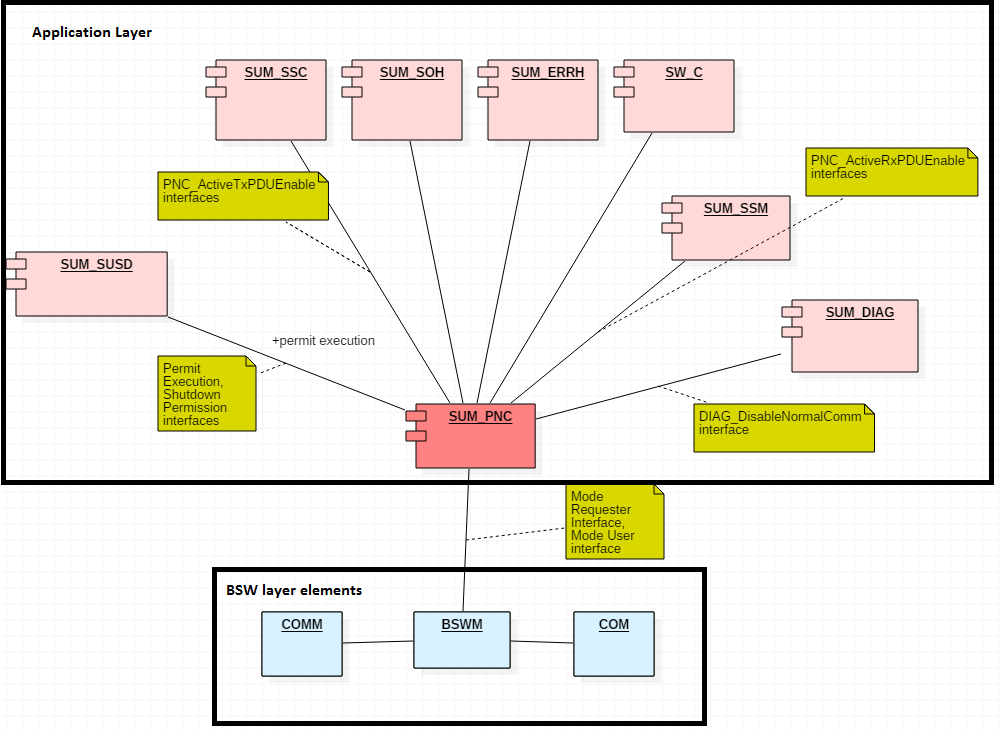
\includegraphics[scale=0.6]{images/stakeholders.png}
\end{figure}

Important stakeholders for this architecture are:

\begin{itemize}
	\item SUM Modules: SUSD, SSC, SOH, ERRH, SSFM, DIAG;
	\item BSW Modules: BswM, Com, ComM;
\end{itemize}
\noindent
Following sections will help in understanding each SUM module and BSW module interfacing dependency and functionalities in detail.
\section{Definitions, Acronyms and Abbreviations}

%tables acronymnsAndAbbr
\begin{longtable}{|l|l|}
\hline
\begin{minipage}{0.31\linewidth}\raggedright\vspace{.75ex}{\cellcolor{eTASPurple}\textcolor{white}{\bfseries Definition} }\vspace{.75ex}\end{minipage} & \begin{minipage}{0.63\linewidth}\raggedright\vspace{.75ex}{\cellcolor{eTASPurple}\textcolor{white}{\bfseries  Description} }\vspace{.75ex}\end{minipage}\\
\hline\hline
\endfirsthead
\hline
\begin{minipage}{0.31\linewidth}\raggedright\vspace{.75ex}{\cellcolor{eTASPurple}\textcolor{white}{\bfseries Definition} }\vspace{.75ex}\end{minipage} & \begin{minipage}{0.63\linewidth}\raggedright\vspace{.75ex}{\cellcolor{eTASPurple}\textcolor{white}{\bfseries  Description} }\vspace{.75ex}\end{minipage}\\
\hline\hline
\endhead
\hline
\endfoot
\hline
\endlastfoot
\begin{minipage}{0.31\linewidth}\raggedright\vspace{.75ex}{\cellcolor{eTASGray30} Activating ECU}\vspace{.75ex}\end{minipage} & \begin{minipage}{0.63\linewidth}\raggedright\vspace{.75ex}{\cellcolor{eTASGray30}  ECU assigned to monitor and process PN Activation Criteria. At least one ECU per PN is an Activating ECU, but there may be others (depends on the architecture deployment)}\vspace{.75ex}\end{minipage}\\\hline
\begin{minipage}{0.31\linewidth}\raggedright\vspace{.75ex}{\cellcolor{eTASGray30} Activated ECU}\vspace{.75ex}\end{minipage} & \begin{minipage}{0.63\linewidth}\raggedright\vspace{.75ex}{\cellcolor{eTASGray30}  ECU is a member of an activated PN. All members of networks supporting PNs are capable of being Activated ECUs}\vspace{.75ex}\end{minipage}\\\hline
\begin{minipage}{0.31\linewidth}\raggedright\vspace{.75ex}{\cellcolor{eTASGray30} Activation Criteria}\vspace{.75ex}\end{minipage} & \begin{minipage}{0.63\linewidth}\raggedright\vspace{.75ex}{\cellcolor{eTASGray30} A set of conditions that result in the activation of a PN. These conditions are typically a combination of local inputs and / or serial data signals}\vspace{.75ex}\end{minipage}\\\hline
\begin{minipage}{0.31\linewidth}\raggedright\vspace{.75ex}{\cellcolor{eTASGray30} API}\vspace{.75ex}\end{minipage} & \begin{minipage}{0.63\linewidth}\raggedright\vspace{.75ex}{\cellcolor{eTASGray30}  Application Program Interface}\vspace{.75ex}\end{minipage}\\\hline
\begin{minipage}{0.31\linewidth}\raggedright\vspace{.75ex}{\cellcolor{eTASGray30} AMM}\vspace{.75ex}\end{minipage} & \begin{minipage}{0.63\linewidth}\raggedright\vspace{.75ex}{\cellcolor{eTASGray30}  Application Mode Manager}\vspace{.75ex}\end{minipage}\\\hline
\begin{minipage}{0.31\linewidth}\raggedright\vspace{.75ex}{\cellcolor{eTASGray30} BSW}\vspace{.75ex}\end{minipage} & \begin{minipage}{0.63\linewidth}\raggedright\vspace{.75ex}{\cellcolor{eTASGray30}  Basic Software}\vspace{.75ex}\end{minipage}\\\hline
\begin{minipage}{0.31\linewidth}\raggedright\vspace{.75ex}{\cellcolor{eTASGray30} BswM}\vspace{.75ex}\end{minipage} & \begin{minipage}{0.63\linewidth}\raggedright\vspace{.75ex}{\cellcolor{eTASGray30}  Basic Software Mode Manager}\vspace{.75ex}\end{minipage}\\\hline
\begin{minipage}{0.31\linewidth}\raggedright\vspace{.75ex}{\cellcolor{eTASGray30} CAN}\vspace{.75ex}\end{minipage} & \begin{minipage}{0.63\linewidth}\raggedright\vspace{.75ex}{\cellcolor{eTASGray30}  Controller Area Network}\vspace{.75ex}\end{minipage}\\\hline
\begin{minipage}{0.31\linewidth}\raggedright\vspace{.75ex}{\cellcolor{eTASGray30} Com}\vspace{.75ex}\end{minipage} & \begin{minipage}{0.63\linewidth}\raggedright\vspace{.75ex}{\cellcolor{eTASGray30}  Communication Module}\vspace{.75ex}\end{minipage}\\\hline
\begin{minipage}{0.31\linewidth}\raggedright\vspace{.75ex}{\cellcolor{eTASGray30} Dcm}\vspace{.75ex}\end{minipage} & \begin{minipage}{0.63\linewidth}\raggedright\vspace{.75ex}{\cellcolor{eTASGray30}  Diagnostic Communication Module}\vspace{.75ex}\end{minipage}\\\hline
\begin{minipage}{0.31\linewidth}\raggedright\vspace{.75ex}{\cellcolor{eTASGray30} Deactivation Criteria}\vspace{.75ex}\end{minipage} & \begin{minipage}{0.63\linewidth}\raggedright\vspace{.75ex}{\cellcolor{eTASGray30}  A set of conditions that result in the deactivation of a PN}\vspace{.75ex}\end{minipage}\\\hline
\begin{minipage}{0.31\linewidth}\raggedright\vspace{.75ex}{\cellcolor{eTASGray30} DTC}\vspace{.75ex}\end{minipage} & \begin{minipage}{0.63\linewidth}\raggedright\vspace{.75ex}{\cellcolor{eTASGray30}  Diagnostic Trouble Code}\vspace{.75ex}\end{minipage}\\\hline
\begin{minipage}{0.31\linewidth}\raggedright\vspace{.75ex}{\cellcolor{eTASGray30} DIAG}\vspace{.75ex}\end{minipage} & \begin{minipage}{0.63\linewidth}\raggedright\vspace{.75ex}{\cellcolor{eTASGray30}  Diagnostic Application Services}\vspace{.75ex}\end{minipage}\\\hline
\begin{minipage}{0.31\linewidth}\raggedright\vspace{.75ex}{\cellcolor{eTASGray30} DFD}\vspace{.75ex}\end{minipage} & \begin{minipage}{0.63\linewidth}\raggedright\vspace{.75ex}{\cellcolor{eTASGray30}  Data Flow Diagram}\vspace{.75ex}\end{minipage}\\\hline
\begin{minipage}{0.31\linewidth}\raggedright\vspace{.75ex}{\cellcolor{eTASGray30} ECU}\vspace{.75ex}\end{minipage} & \begin{minipage}{0.63\linewidth}\raggedright\vspace{.75ex}{\cellcolor{eTASGray30}  Electronic Control Unit}\vspace{.75ex}\end{minipage}\\\hline
\begin{minipage}{0.31\linewidth}\raggedright\vspace{.75ex}{\cellcolor{eTASGray30} Ecuc}\vspace{.75ex}\end{minipage} & \begin{minipage}{0.63\linewidth}\raggedright\vspace{.75ex}{\cellcolor{eTASGray30}  ECU Configuration File}\vspace{.75ex}\end{minipage}\\\hline
\begin{minipage}{0.31\linewidth}\raggedright\vspace{.75ex}{\cellcolor{eTASGray30} ERRH}\vspace{.75ex}\end{minipage} & \begin{minipage}{0.63\linewidth}\raggedright\vspace{.75ex}{\cellcolor{eTASGray30}  Error Handling Module}\vspace{.75ex}\end{minipage}\\\hline
\begin{minipage}{0.31\linewidth}\raggedright\vspace{.75ex}{\cellcolor{eTASGray30} FSM}\vspace{.75ex}\end{minipage} & \begin{minipage}{0.63\linewidth}\raggedright\vspace{.75ex}{\cellcolor{eTASGray30}  Finite State Machine}\vspace{.75ex}\end{minipage}\\\hline
\begin{minipage}{0.31\linewidth}\raggedright\vspace{.75ex}{\cellcolor{eTASGray30} GM}\vspace{.75ex}\end{minipage} & \begin{minipage}{0.63\linewidth}\raggedright\vspace{.75ex}{\cellcolor{eTASGray30}  General Motors}\vspace{.75ex}\end{minipage}\\\hline
\begin{minipage}{0.31\linewidth}\raggedright\vspace{.75ex}{\cellcolor{eTASGray30} Locally Active PN}\vspace{.75ex}\end{minipage} & \begin{minipage}{0.63\linewidth}\raggedright\vspace{.75ex}{\cellcolor{eTASGray30}  PN that is activated from within the ECU because its PN Activation Criteria was met}\vspace{.75ex}\end{minipage}\\\hline
\begin{minipage}{0.31\linewidth}\raggedright\vspace{.75ex}{\cellcolor{eTASGray30} PNC}\vspace{.75ex}\end{minipage} & \begin{minipage}{0.63\linewidth}\raggedright\vspace{.75ex}{\cellcolor{eTASGray30}  Partial Network Coordinator}\vspace{.75ex}\end{minipage}\\\hline
\begin{minipage}{0.31\linewidth}\raggedright\vspace{.75ex}{\cellcolor{eTASGray30} Remotely Active PN}\vspace{.75ex}\end{minipage} & \begin{minipage}{0.63\linewidth}\raggedright\vspace{.75ex}{\cellcolor{eTASGray30}  PN that is activated from outside the ECU}\vspace{.75ex}\end{minipage}\\\hline
\begin{minipage}{0.31\linewidth}\raggedright\vspace{.75ex}{\cellcolor{eTASGray30} SOH}\vspace{.75ex}\end{minipage} & \begin{minipage}{0.63\linewidth}\raggedright\vspace{.75ex}{\cellcolor{eTASGray30}  State Of Health Manager}\vspace{.75ex}\end{minipage}\\\hline
\begin{minipage}{0.31\linewidth}\raggedright\vspace{.75ex}{\cellcolor{eTASGray30} SSFM}\vspace{.75ex}\end{minipage} & \begin{minipage}{0.63\linewidth}\raggedright\vspace{.75ex}{\cellcolor{eTASGray30}  Signal Status adn Fault Monitor}\vspace{.75ex}\end{minipage}\\\hline
\begin{minipage}{0.31\linewidth}\raggedright\vspace{.75ex}{\cellcolor{eTASGray30} SSC}\vspace{.75ex}\end{minipage} & \begin{minipage}{0.63\linewidth}\raggedright\vspace{.75ex}{\cellcolor{eTASGray30}  Security Service Coordinator}\vspace{.75ex}\end{minipage}\\\hline
\begin{minipage}{0.31\linewidth}\raggedright\vspace{.75ex}{\cellcolor{eTASGray30} SUM}\vspace{.75ex}\end{minipage} & \begin{minipage}{0.63\linewidth}\raggedright\vspace{.75ex}{\cellcolor{eTASGray30}  Standard Utility Module}\vspace{.75ex}\end{minipage}\\\hline
\begin{minipage}{0.31\linewidth}\raggedright\vspace{.75ex}{\cellcolor{eTASGray30} SUSD}\vspace{.75ex}\end{minipage} & \begin{minipage}{0.63\linewidth}\raggedright\vspace{.75ex}{\cellcolor{eTASGray30}  Startup Shut down Coordinator}\vspace{.75ex}\end{minipage}\\\hline
\begin{minipage}{0.31\linewidth}\raggedright\vspace{.75ex}{\cellcolor{eTASGray30} SW-C}\vspace{.75ex}\end{minipage} & \begin{minipage}{0.63\linewidth}\raggedright\vspace{.75ex}{\cellcolor{eTASGray30}  Software Component}\vspace{.75ex}\end{minipage}\\\hline
\begin{minipage}{0.31\linewidth}\raggedright\vspace{.75ex}{\cellcolor{eTASGray30} SW or S/W}\vspace{.75ex}\end{minipage} & \begin{minipage}{0.63\linewidth}\raggedright\vspace{.75ex}{\cellcolor{eTASGray30}  Software}\vspace{.75ex}\end{minipage}\\\hline
\begin{minipage}{0.31\linewidth}\raggedright\vspace{.75ex}{\cellcolor{eTASGray30} VMM}\vspace{.75ex}\end{minipage} & \begin{minipage}{0.63\linewidth}\raggedright\vspace{.75ex}{\cellcolor{eTASGray30}  Vehicle Mode Manager}\vspace{.75ex}\end{minipage}\\\hline
\begin{minipage}{0.31\linewidth}\raggedright\vspace{.75ex}{\cellcolor{eTASGray30} WRT/wrt}\vspace{.75ex}\end{minipage} & \begin{minipage}{0.63\linewidth}\raggedright\vspace{.75ex}{\cellcolor{eTASGray30}  With respect to }\vspace{.75ex}\end{minipage}\\\hline
\end{longtable}

\section{Referenced Documents}

\begin{longtable}{|l|l|l|l|}
\hline
\begin{minipage}{0.42\linewidth}\raggedright\vspace{.75ex}{\cellcolor{eTASPurple}\textcolor{white}{\bfseries Document Name} }\vspace{.75ex}\end{minipage} & \begin{minipage}{0.18\linewidth}\raggedright\vspace{.75ex}{\cellcolor{eTASPurple}\textcolor{white}{\bfseries Description} }\vspace{.75ex}\end{minipage} & \begin{minipage}{0.15\linewidth}\raggedright\vspace{.75ex}{\cellcolor{eTASPurple}\textcolor{white}{\bfseries Version} }\vspace{.75ex}\end{minipage} & \begin{minipage}{0.13\linewidth}\raggedright\vspace{.75ex}{\cellcolor{eTASPurple}\textcolor{white}{\bfseries Release Date} }\vspace{.75ex}\end{minipage}\\
\hline\hline
\endfirsthead
\hline
\begin{minipage}{0.42\linewidth}\raggedright\vspace{.75ex}{\cellcolor{eTASPurple}\textcolor{white}{\bfseries Document Name} }\vspace{.75ex}\end{minipage} & \begin{minipage}{0.18\linewidth}\raggedright\vspace{.75ex}{\cellcolor{eTASPurple}\textcolor{white}{\bfseries Description} }\vspace{.75ex}\end{minipage} & \begin{minipage}{0.15\linewidth}\raggedright\vspace{.75ex}{\cellcolor{eTASPurple}\textcolor{white}{\bfseries Version} }\vspace{.75ex}\end{minipage} & \begin{minipage}{0.13\linewidth}\raggedright\vspace{.75ex}{\cellcolor{eTASPurple}\textcolor{white}{\bfseries Release Date} }\vspace{.75ex}\end{minipage}\\
\hline\hline
\endhead
\hline
\endfoot
\hline
\endlastfoot
\begin{minipage}{0.42\linewidth}\raggedright\vspace{.75ex}{\cellcolor{eTASGray30} SDV-8002 AUTOSAR Standard Utility Modules Specification}\vspace{.75ex}\end{minipage} & \begin{minipage}{0.18\linewidth}\raggedright\vspace{.75ex}{\cellcolor{eTASGray30} PNC module specification}\vspace{.75ex}\end{minipage} & \begin{minipage}{0.15\linewidth}\raggedright\vspace{.75ex}{\cellcolor{eTASGray30} 27.27.180.3p0}\vspace{.75ex}\end{minipage} & \begin{minipage}{0.13\linewidth}\raggedright\vspace{.75ex}{\cellcolor{eTASGray30} 04/04/2025}\vspace{.75ex}\end{minipage}\\\hline
\begin{minipage}{0.42\linewidth}\raggedright\vspace{.75ex}{\cellcolor{eTASGray30} GB5280 GLobal B Partial Network Deployment Specification}\vspace{.75ex}\end{minipage} & \begin{minipage}{0.18\linewidth}\raggedright\vspace{.75ex}{\cellcolor{eTASGray30} Partial Network deployment specification}\vspace{.75ex}\end{minipage} & \begin{minipage}{0.15\linewidth}\raggedright\vspace{.75ex}{\cellcolor{eTASGray30} MY25.162}\vspace{.75ex}\end{minipage} & \begin{minipage}{0.13\linewidth}\raggedright\vspace{.75ex}{\cellcolor{eTASGray30} 09/09/2021}\vspace{.75ex}\end{minipage}\\\hline
\begin{minipage}{0.42\linewidth}\raggedright\vspace{.75ex}{\cellcolor{eTASGray30} SDV-6001 Diagnostic Infrastructure Specification}\vspace{.75ex}\end{minipage} & \begin{minipage}{0.18\linewidth}\raggedright\vspace{.75ex}{\cellcolor{eTASGray30} PNC DIDs specification}\vspace{.75ex}\end{minipage} & \begin{minipage}{0.15\linewidth}\raggedright\vspace{.75ex}{\cellcolor{eTASGray30} 27.27.180.3p0}\vspace{.75ex}\end{minipage} & \begin{minipage}{0.13\linewidth}\raggedright\vspace{.75ex}{\cellcolor{eTASGray30} 04/09/2025}\vspace{.75ex}\end{minipage}\\\hline
\end{longtable}